% Provenance (never printed): see sources/outline_sources.md (Year 2: metamorphic reactions,
% Clapeyron slopes, the Al2SiO5 diagram, the facies grid, protoliths). Definitions and facies
% table from the IUGS subcommission proposal (via the Granada translation); thermodynamic data
% from Robie and Hemingway (1995); experimental diagram from Holdaway and Mukhopadhyay (1993);
% curves from figdata/bachelor-2/facies.py; exercise and problem values in the Book 4 scratch
% calculator calc/ch10.py.
\chapter{变质反应与变质相}\label{ch:b2:metamorphic-facies}

随板块下沉的玄武岩不会保持为玄武岩。其斜长石和辉石
在固态下转变为其他矿物，新的\omterm{def:b2:metamorphic-facies:assemblage}{矿物组合}取决于其所经历的
压力和温度：形成由蓝闪石和硬柱石组成的蓝色岩石，或
由绿辉石和石榴子石组成的绿红色岩石。变质岩返回地表时仍保留这些矿物，
懂得这些反应的岩石学家可以反推其
形成条件。本章用化学课程中的热力学方法书写这些反应，
根据实测数据计算最著名的\omterm{def:b2:metamorphic-facies:facies}{变质相图}，
即三种 \ce{Al2SiO5} 矿物的相图，与实验相比较，并
将变质岩的\omterm{def:b2:metamorphic-facies:assemblage}{矿物组合}归纳为\omterm{def:b2:metamorphic-facies:facies}{变质相}。
% ledger: scmr:facies-assemblages

\begin{recall}
\textbf{来自高中分册}：\omterm{def:b2:metamorphic-facies:metamorphism}{变质作用}、变质级、指示矿物
等变质线、接触\omterm{def:b2:metamorphic-facies:metamorphism}{变质作用}及其\omterm{def:b2:magma-emplacement:aureole}{接触变质晕}、面理和片理、
静岩压力；蓝晶石、红柱石和夕线石作为同质多象变体，及其
相图。\textbf{来自物理与化学系列的本科一年级分册}：吉布斯
自由能 $G = H - TS$，其极小值标志着给定 $T$ 和 $P$ 时的稳定态；
焓、熵和热容；$\mathrm dG = V\,\mathrm dP - S\,\mathrm dT$；
以及纯净物汽化的克劳修斯–克拉珀龙关系和水的三
相点。\textbf{来自本科一年级分册}：俯冲带、碰撞带和
地温线。
\end{recall}

\section{变质作用}\label{sec:b2:metamorphic-facies:metamorphism}

高中分册把\omterm{def:b2:metamorphic-facies:metamorphism}{变质作用}看作岩石在热和
压力作用下的转变。本书采用国际推荐的定义。

\begin{definition}[变质作用；原岩]\label{def:b2:metamorphic-facies:metamorphism}
\emph{变质作用}\index{变质作用}是一种过程，它改变岩石的矿物或微观结构，或两者兼而有之，
主要在固态下进行，使岩石适应与其形成时不同、
也不同于地表及成岩带中通常所见的物理条件。
它可以与\omterm{def:b2:mantle-melting:melting}{部分熔融}并存，
并可改变岩石的化学组成。变质前的
岩石即为其\emph{原岩}\index{原岩}。
\end{definition}
% ledger: scmr:metamorphism

下限排除了成岩作用，即沉积物被埋藏和
固结时发生的变化；上限为熔融，在\cref{ch:b2:crustal-melting}中讨论。
作用因素是温度、压力、在岩石中循环的流体（主要是水和
二氧化碳）以及变形。\omterm{def:b2:metamorphic-facies:metamorphism}{变质作用}按其范围和
产出环境进行分类。
% ledger: scmr:metamorphism, scmr:types

\emph{区域}\omterm{def:b2:metamorphic-facies:metamorphism}{变质作用}影响大体积岩石，并伴随大尺度构造
过程：在造山带中为\emph{造山型}，地壳在
碰撞中增厚；\emph{埋藏}\omterm{def:b2:metamorphic-facies:metamorphism}{变质作用}影响深埋于厚层
沉积或火山堆积之下的岩石，不伴随变形或\omterm{def:b2:magma-emplacement:magma}{岩浆}作用，因此其岩石
通常缺乏片理；\emph{洋底}\omterm{def:b2:metamorphic-facies:metamorphism}{变质作用}改变靠近洋中脊的地壳，
热海水在陡峭热梯度下循环穿过地壳，
其重结晶通常不完全。\emph{局部}\omterm{def:b2:metamorphic-facies:metamorphism}{变质作用}
具有局部成因：\emph{接触}\omterm{def:b2:metamorphic-facies:metamorphism}{变质作用}加热侵入体的围岩；
\emph{热液}\omterm{def:b2:metamorphic-facies:metamorphism}{变质作用}由富水热流体驱动；
\emph{错动}\omterm{def:b2:metamorphic-facies:metamorphism}{变质作用}发生在断层和剪切带中，使晶粒变小，
形成糜棱岩和碎裂岩；\emph{冲击}\omterm{def:b2:metamorphic-facies:metamorphism}{变质作用}在\omterm{def:b2:planet-formation-meteorites:fall-find}{陨石}撞击下，
可使岩石熔融和汽化。\omterm{def:b2:metamorphic-facies:metamorphism}{变质作用}在温度升高时称为进变质，
温度下降时称为退变质。
% ledger: scmr:types

\section{变质反应}\label{sec:b2:metamorphic-facies:reactions}

\begin{definition}[变质反应；脱挥发分反应]\label{def:b2:metamorphic-facies:reaction}
\emph{变质反应}\index{变质反应}使岩石中的一组矿物（反应物）
转变为另一组矿物（生成物），在固态下进行，
可有流体相参与。\emph{脱挥发分反应}\index{脱挥发分反应}
是指释放挥发分的反应，即脱水反应释放水，脱碳反应释放
二氧化碳。
\end{definition}

本章将出现三种类型。同质多象转变，例如蓝晶石转变为
夕线石，或方解石转变为文石，二者化学式不变而结构改变。
固体之间的其他反应使组分在矿物之间重新分配，例如
钠长石生成硬玉和石英：
\[
\ce{NaAlSi3O8 -> NaAlSi2O6 + SiO2}.
\]
\omterm{def:b2:metamorphic-facies:reaction}{脱挥发分反应}释放流体，例如白云母与石英
在高温下分解：
\[
\ce{KAl3Si3O10(OH)2 + SiO2 -> KAlSi3O8 + Al2SiO5 + H2O}.
\]
% ledger: day73:ms-qz

对于成分固定的矿物之间的反应，吉布斯自由能的变化为
$\Delta_r G(T, P) = \sum G_{\text{生成物}} - \sum G_{\text{反应物}}$；
生成物在 $\Delta_r G < 0$ 处稳定，反应物在 $\Delta_r G > 0$ 处稳定，
二者在 $\Delta_r G = 0$ 处共存。

\begin{definition}[单变反应]\label{def:b2:metamorphic-facies:univariant}
成分固定的相之间的反应称为\emph{单变反应}\index{单变反应}，
当其平衡条件 $\Delta_r G(T, P) = 0$ 只留下一个自由变量时，
平衡在压力–温度平面中为一条线，该线把反应物的
区域与生成物的区域分开。
\end{definition}

\begin{definition}[克拉珀龙斜率]\label{def:b2:metamorphic-facies:clapeyron}
反应的\emph{克拉珀龙斜率}\index{克拉珀龙斜率}是
其平衡线在压力–温度平面中的斜率 $\mathrm dP/\mathrm dT$。
\end{definition}

\begin{proposition}[反应的克拉珀龙斜率]\label{prop:b2:metamorphic-facies:clapeyron}
对于熵变为 $\Delta_r S$、体积变化为
$\Delta_r V$ 的反应，其平衡线上有
\[
\frac{\mathrm dP}{\mathrm dT} = \frac{\Delta_r S}{\Delta_r V}.
\]
\end{proposition}

\begin{proof}
对每一相有 $\mathrm dG = V\,\mathrm dP - S\,\mathrm dT$，于是对该反应
$\mathrm d(\Delta_r G) = \Delta_r V\,\mathrm dP - \Delta_r S\,\mathrm dT$。沿此线
$\Delta_r G = 0$ 保持为零：$\Delta_r V\,\mathrm dP = \Delta_r S\,\mathrm dT$。
\end{proof}

这是物理学中的克劳修斯–克拉珀龙关系，此处针对固体写出。
取 $\Delta_r S$ 以 \unit{J.mol^{-1}.K^{-1}} 计、$\Delta_r V$ 以 \unit{J.bar^{-1}} 计（一
\unit{J.bar^{-1}} 即 \qty{10}{cm^3}），斜率以 bar/K 计。两
条推论决定了每一张\omterm{def:b2:metamorphic-facies:facies}{变质相图}的形态。固体之间，熵变与体积变化
都很小，因此反应线可陡可缓，可正可负
：高温一侧为熵较大的产物，而
高压一侧为体积较小的产物。在\omterm{def:b2:metamorphic-facies:reaction}{脱挥发分反应}中，流体带来很大的熵，
因此产物位于高温一侧；流体的体积在低压时很大，
随压力升高而缩小，使斜率在低压时较缓、
高压时较陡。反应线因此弯曲。
白云母与石英的实验表明，该线在 1、2 和 \qty{3}{kbar} 的水压力下，
分别位于 603、637 和 \qty{662}{\celsius}；1 至 \qty{2}{kbar} 之间，该线每开尔文升高
\qty{29}{bar}，2 至 \qty{3}{kbar} 之间为 \qty{40}{bar}（见\cref{exo:b2:metamorphic-facies:9}）。
% ledger: day73:ms-qz

\section{铝硅酸盐}\label{sec:b2:metamorphic-facies:al2sio5}

\begin{definition}[铝硅酸盐同质多象变体]\label{def:b2:metamorphic-facies:al2sio5}
称\emph{铝硅酸盐同质多象变体}\index{铝硅酸盐同质多象变体}为化学式为 \ce{Al2SiO5} 的三种
矿物：蓝晶石（三斜），红柱石和夕线石（两者同属
斜方晶系）。
\end{definition}
% ledger: rh95:al2sio5

它们常见于变质泥岩中，并携带泥岩中的铝。由于三者化学式相同，
生成哪一种仅取决于压力与温度。下表
给出了它们的实测性质。

\begin{center}
\small
\begin{tabular}{@{}lrrrr@{}}
\hline
 & $\Delta_f H^\circ$ (\unit{kJ.mol^{-1}}) & $S^\circ$ (\unit{J.mol^{-1}.K^{-1}}) & $V^\circ$ (\unit{J.bar^{-1}}) & 密度 (\unit{g.cm^{-3}})\\
\hline
蓝晶石 & $-2593.8$ & 82.80 & 4.415 & 3.670\\
红柱石 & $-2589.9$ & 91.39 & 5.152 & 3.145\\
夕线石 & $-2586.1$ & 95.40 & 4.986 & 3.250\\
\hline
\end{tabular}
\par\smallskip{\small 蓝晶石、红柱石和夕线石在 \qty{298.15}{K} 和
\qty{1}{bar} 下的数据（Robie and Hemingway, 1995）；焓的不确定度为
\qty{2.0}{kJ.mol^{-1}}，熵的不确定度为 0.5。密度由摩尔质量
\qty{162.046}{g.mol^{-1}} 与体积求得。}
\end{center}
% ledger: rh95:al2sio5

蓝晶石密度最大、熵最小，是高压、
低温的同质多象变体。红柱石密度最小，对应低压；夕线石
熵最大，对应高温。它们的平衡线可以算出。

\begin{method}[计算反应线]\label{met:b2:metamorphic-facies:line}
(1) 由表中数据求出 $\Delta_r H$、$\Delta_r S$ 与 $\Delta_r V$，取 \qty{298.15}{K}
和 \qty{1}{bar}。(2) 忽略 $\Delta_r H$ 与 $\Delta_r S$ 随
温度的变化（产物与反应物的热容近似相等），以及 $\Delta_r V$ 随
压力和温度的变化（固体几乎不压缩或膨胀）：
\[
\Delta_r G(T, P) \approx \Delta_r H - T\,\Delta_r S + \Delta_r V\,(P - 1).
\]
(3) 令其为零：$P = 1 + (T\,\Delta_r S - \Delta_r H)/\Delta_r V$，这是一条
斜率为 $\Delta_r S/\Delta_r V$ 的直线。(4) 精度要求较高时，将 $\Delta_r H$ 与
$\Delta_r S$ 换成温度 $T$ 下的值，取自 $H_T - H_{298}$ 与 $S_T$ 的表，
再重新求解。(5) 对每条线，只保留其两相
比任何第三相都更稳定的部分。
\end{method}

对蓝晶石到红柱石，$\Delta_r H = \qty{3.9}{kJ}$，$\Delta_r S =
\qty{8.59}{J.K^{-1}}$，$\Delta_r V = \qty{0.737}{J.bar^{-1}}$：在 \qty{25}{\celsius}
和 \qty{1}{bar}，$\Delta_r G = 3900 - 298.15\times8.59 = \qty{+1.34}{kJ}$，故蓝晶石而非红柱石
是地表稳定的同质多象变体；蓝晶石到夕线石在该处
有 $\Delta_r G = \qty{+3.94}{kJ}$。各斜率分别为：蓝晶石到红柱石 $8.59/0.737 = \qty{11.7}{bar/K}$，
蓝晶石到夕线石 $12.60/0.571 = \qty{22.1}{bar/K}$，
红柱石到夕线石 $4.01/(-0.166) = \qty{-24.2}{bar/K}$，在三者中，
只有这一反应的高温一侧产物密度更大。
% ledger: rh95:al2sio5

\begin{definition}[不变点]\label{def:b2:metamorphic-facies:invariant}
称\emph{不变点}\index{不变点}为压力–温度平面中的一点，在该点体系的
三个或更多相平衡共存，且其间每条\omterm{def:b2:metamorphic-facies:univariant}{单变}线都交于此点；
该点上没有自由变量。
\end{definition}

\begin{proposition}[三相点]\label{prop:b2:metamorphic-facies:triple}
三条线，蓝晶石 $=$ 红柱石、蓝晶石 $=$ 夕线石与红柱石 $=$
夕线石，交于一点。在该点附近，每条线只在一侧稳定；其
亚稳延伸部分位于第三种同质多象变体的稳定场内。
\end{proposition}

\begin{proof}
对任意 $(T, P)$，$\Delta G_{\text{ky}\to\text{sil}} = \Delta G_{\text{ky}\to\text{and}} +
\Delta G_{\text{and}\to\text{sil}}$，因红柱石的吉布斯能相互抵消。在前两条线相交处，
两项为零，故第三项亦为零：第三条线
经过交点。越过交点后，以蓝晶石 $=$ 红柱石这条线为例，
即 $G_{\text{ky}} = G_{\text{and}}$，但该点位于其余两条线的夕线石一侧，
故 $G_{\text{sil}}$ 小于二者：蓝晶石与红柱石在该处都不稳定，
因此该线是亚稳的。
\end{proof}

若按方法中的常数性质计算，三相点位于
\qty{514}{\celsius} 和 \qty{3.88}{kbar}（周末问题）；若计入表中数据的温度依赖性，则位于
\qty{536}{\celsius} 和 \qty{4.20}{kbar}。由逆转实验绘制的实验相图
给出其位于 $504 \pm \qty{20}{\celsius}$ 和
$3.75 \pm \qty{0.25}{kbar}$（见下图）。
% ledger: rh95:al2sio5-ht, hm93:triple, hm93:table11

\begin{omfigure}
\centering
\begin{tikzpicture}
\begin{axis}[omrecord, width=0.84\linewidth, height=7.4cm,
  xmin=200, xmax=900, ymin=0, ymax=10, xlabel={$T$ (\unit{\celsius})}, ylabel={$P$ (\unit{kbar})},
  legend style={font=\scriptsize, at={(0.02,0.98)}, anchor=north west},
  tick label style={font=\scriptsize}, label style={font=\small}]
\addplot[very thick, blue!70!black] table[x=T_C, y=P_kbar] {figdata/out/bachelor-2-facies-stable-kyand.dat};
\addlegendentry{计算值（据表）}
\addplot[thick, gray, densely dashed, mark=o, mark size=1.2pt] table[x=T_C, y=P_kbar] {figdata/out/bachelor-2-facies-hm93-kyand.dat};
\addlegendentry{实验}
\addplot[thick, orange!85!black, mark=square*, mark size=1.3pt] table[x=T_C, y=P_kbar] {figdata/out/bachelor-2-facies-day73.dat};
\addlegendentry{白云母 + 石英}
\addplot[very thick, blue!70!black, forget plot] table[x=T_C, y=P_kbar] {figdata/out/bachelor-2-facies-stable-kysil.dat};
\addplot[very thick, blue!70!black, forget plot] table[x=T_C, y=P_kbar] {figdata/out/bachelor-2-facies-stable-andsil.dat};
\addplot[thin, blue!70!black, dashed, forget plot] table[x=T_C, y=P_kbar] {figdata/out/bachelor-2-facies-meta-kyand.dat};
\addplot[thin, blue!70!black, dashed, forget plot] table[x=T_C, y=P_kbar] {figdata/out/bachelor-2-facies-meta-kysil.dat};
\addplot[thin, blue!70!black, dashed, forget plot] table[x=T_C, y=P_kbar] {figdata/out/bachelor-2-facies-meta-andsil.dat};
\addplot[thick, gray, densely dashed, mark=o, mark size=1.2pt, forget plot] table[x=T_C, y=P_kbar] {figdata/out/bachelor-2-facies-hm93-kysil.dat};
\addplot[thick, gray, densely dashed, mark=o, mark size=1.2pt, forget plot] table[x=T_C, y=P_kbar] {figdata/out/bachelor-2-facies-hm93-andsil.dat};
\addplot[only marks, mark=*, mark size=2pt, blue!70!black, forget plot] table[x=T_C, y=P_kbar] {figdata/out/bachelor-2-facies-triple-B.dat};
\addplot[only marks, mark=*, mark size=2pt, gray, forget plot] table[x=T_C, y=P_kbar] {figdata/out/bachelor-2-facies-hm93-triple.dat};
\node[font=\small\bfseries] at (axis cs:330,6.2) {蓝晶石};
\node[font=\small\bfseries] at (axis cs:460,0.6) {红柱石};
\node[font=\small\bfseries] at (axis cs:790,3.6) {夕线石};
\end{axis}
\end{tikzpicture}
\par\smallskip{\small 由 Robie 和 Hemingway（1995）热力学数据表计算的 \ce{Al2SiO5} 相图，
计入焓与熵随温度的变化（蓝色；虚线：亚稳延伸），
以及 Holdaway 和 Mukhopadhyay（1993）的实验相图
（灰色，示其表列数据点）。橙色：Day（1973）测得的白云母 + 石英分解，
该曲线有弯折。}
\end{omfigure}
% ledger: rh95:al2sio5, rh95:al2sio5-ht, hm93:table11, hm93:triple, day73:ms-qz

计算得到的蓝晶石–红柱石线在 400 至 \qty{600}{\celsius} 之间，
与实验线的差别不超过 \qty{0.1}{kbar}；而红柱石–夕线石线在
\qty{600}{\celsius} 处偏高 \qty{0.65}{kbar}。该线是三条线中最脆弱的一条：
其中 $\Delta_r V = \qty{-0.166}{J.bar^{-1}}$，$\Delta_r H$ 只要有 \qty{0.1}{kJ} 的误差，
这仅相当于表中每个焓值不确定度的二十分之一，便足以使该线移动
\qty{600}{bar}。表中的焓值本身是为拟合实验而在其不确定度范围内调整的，
因此决定相图的是实验，而非量热测定。
——相图由实验而非量热法单独确定。
% ledger: rh95:al2sio5, hm93:adjusted, hm93:table11

下图说明为何相线是一条边界。在 \qty{6}{kbar} 下，红柱石与夕线石的吉布斯能
以蓝晶石为基准，两者的吉布斯能在各自变得比蓝晶石更稳定的位置与零线相交；
两者之差从未超过每摩尔几千焦，
这正是焓的微小误差会使相线移动如此之远的原因。

\begin{omfigure}
\centering
\begin{tikzpicture}
\begin{axis}[omrecord, width=0.7\linewidth, height=5.4cm,
  xmin=300, xmax=900, ymin=-4, ymax=4.5, xlabel={$T$ (\unit{\celsius})},
  ylabel={$G - G_{\text{蓝晶石}}$ (\unit{kJ.mol^{-1}})},
  legend style={font=\scriptsize, at={(0.02,0.02)}, anchor=south west},
  tick label style={font=\scriptsize}, label style={font=\small}]
\addplot[very thick, red!75!black] table[x=T_C, y=dG_and] {figdata/out/bachelor-2-facies-dg6.dat};
\addlegendentry{红柱石}
\addplot[very thick, green!45!black] table[x=T_C, y=dG_sil] {figdata/out/bachelor-2-facies-dg6.dat};
\addlegendentry{夕线石}
\addplot[thin, black] coordinates {(300,0) (900,0)};
\end{axis}
\end{tikzpicture}
\par\smallskip{\small 红柱石和夕线石相对于蓝晶石的吉布斯能，取自同一套表，压强为
\qty{6}{kbar}。两曲线均为正时蓝晶石稳定；
夕线石在 \qty{624}{\celsius} 时取而代之。红柱石仅在
\qty{692}{\celsius} 时穿过零线，此时夕线石已更低。高于三相点压强时，
红柱石从不是最稳定的相。}
\end{omfigure}
% ledger: rh95:al2sio5, rh95:al2sio5-ht

\begin{inthelab}[反应的逆转]
反应线是在实验室中通过固定压强与温度下的实验确定的，实验起始物为
反应物与产物的混合物。在活塞–圆筒装置中，将混合物保持一至数天；
然后由 X 射线衍射判定反应方向：比较产物与反应物的峰强比，
并与起始混合物的比值对照，且以稳定矿物上的外延生长加以确认。
另一些研究将红柱石单晶置于蓝晶石或夕线石粉末中反应，并称重，
所用微量天平的精度约为 \qty{4}{\micro g}。
当平衡线两侧都观察到双方各自的生长时，该平衡称为\emph{可逆的}，
线位于两者之间的区间内，
区间宽度由仪器误差决定，通常为 \qty{10}{\celsius} 与 \qty{0.5}{kbar}。
实验者判断相图时，首先依据这类逆转实验，
其次才依据岩石。
\end{inthelab}
% ledger: hm93:methods

\section{矿物组合与变质相}\label{sec:b2:metamorphic-facies:facies}

\begin{definition}[矿物组合]\label{def:b2:metamorphic-facies:assemblage}
称\emph{矿物组合}\index{矿物组合}为在变质岩中
于平衡条件下共同生长的矿物的集合。
\end{definition}

\omterm{def:b2:metamorphic-facies:assemblage}{矿物组合}取决于变质条件以及岩石的
化学组成。埃斯科拉于 1915 年提出了\omterm{def:b2:metamorphic-facies:facies}{变质相}的概念，他看到
同一化学组成的岩石在相同条件下具有相同的组合，
不同岩石的组合在条件变化时同步变化；
国际上的建议保留了他的这一概念。
% ledger: scmr:facies

\begin{definition}[变质相；变质相图]\label{def:b2:metamorphic-facies:facies}
称\emph{变质相}\index{变质相}为一组变质\omterm{def:b2:metamorphic-facies:assemblage}{矿物
组合}，它们在时间和空间上反复共生，并显示出矿物成分与
全岩化学组成之间的规律关系，使得不同的相
对应于不同的变质条件，主要是温度和压强。
变质相是根据玄武质岩石的组合命名和定义的。
\emph{变质相图}\index{变质相图}是各变质相在
压强–温度平面上的排列。
\end{definition}
% ledger: scmr:facies

下表按变玄武岩中的特征矿物列出十种\omterm{def:b2:metamorphic-facies:facies}{变质相}。

\begin{center}
\small
\begin{tabular}{@{}p{0.27\linewidth}p{0.66\linewidth}@{}}
\hline
\omterm{def:b2:metamorphic-facies:facies}{变质相} & 变玄武岩的特征矿物 \\
\hline
沸石相 & 如浊沸石和斜发沸石等沸石类矿物 \\
葡萄石–绿纤石相 & 葡萄石 + 绿纤石、葡萄石 + 阳起石、绿纤石 + 阳起石 \\
绿片岩相 & 阳起石 + 钠长石 + 绿泥石 + 绿帘石 \\
绿帘角闪岩相 & 普通角闪石 + 钠长石 + 绿帘石 $\pm$ 绿泥石 \\
角闪岩相 & 普通角闪石 + 斜长石（钙长石含量超过 \qty{17}{\percent}）\\
麻粒岩相 & 单斜辉石 + 斜方辉石 + 斜长石；橄榄石不能与斜长石或石榴子石稳定共存 \\
蓝片岩相 & 蓝闪石 + 绿帘石 $\pm$ 石榴子石，或蓝闪石 + 硬柱石 \\
榴辉岩相 & 绿辉石 + 石榴子石；斜长石不稳定 \\
辉石\omterm{def:b2:magma-emplacement:aureole}{角岩}相 & 单斜辉石 + 斜方辉石 + 斜长石；橄榄石与斜长石稳定共存 \\
砂晶岩相 & 同上，并含易变辉石等极高温矿物 \\
\hline
\end{tabular}
\par\smallskip{\small 玄武质岩石中的各\omterm{def:b2:metamorphic-facies:facies}{变质相}及其特征\omterm{def:b2:metamorphic-facies:assemblage}{矿物组合}，
依据国际推荐方案（埃斯科拉的八个相，
沸石相和葡萄石–绿纤石相为后来补充）。}
\end{center}
% ledger: scmr:facies-assemblages, scmr:facies

推荐方案着重说明\omterm{def:b2:metamorphic-facies:facies}{变质相}不做什么：它们记录的是\omterm{def:b2:metamorphic-facies:assemblage}{矿物组合}之间的规律，
而不试图确定每一相的压强和温度。各相在
压强–温度平面中的排列次序由它们之间的反应决定，
下图示意性地画出了这一次序。温度由沸石相
经绿片岩相和角闪岩相升至麻粒岩相；低压高温处为
\omterm{def:b2:magma-emplacement:aureole}{接触变质晕}的\omterm{def:b2:magma-emplacement:aureole}{角岩}相；高压低温处为
蓝片岩相；高压较高温处为榴辉岩相。
本章的反应界定了边界的一部分：斜长石，
自绿片岩相至麻粒岩相以钠长石或钙质更高的斜长石形式存在，在榴辉岩相中不稳定，
正如其钠长石转变为硬玉和石英时那样（见\cref{exo:b2:metamorphic-facies:8}）；方解石
在高压下转变为
更致密的文石（见\cref{exo:b2:metamorphic-facies:7}）。
% ledger: scmr:facies, scmr:facies-assemblages

\begin{omfigure}
\centering
\begin{tikzpicture}[font=\scriptsize, x=1cm, y=1cm]
\draw[->, thick] (0,0) -- (9.4,0) node[below left] {温度};
\draw[->, thick] (0,0) -- (0,6.4) node[above right] {压强（深度）};
\fill[orange!12] (0.3,0.1) -- (1.4,0.1) -- (1.4,1.8) -- (0.3,1.8) -- cycle;
\fill[orange!20] (1.4,0.1) -- (2.7,0.1) -- (2.7,2.6) -- (1.4,2.6) -- (1.4,1.8) -- cycle;
\fill[green!14] (2.7,0.9) -- (4.4,0.9) -- (4.4,3.6) -- (2.7,3.4) -- cycle;
\fill[green!24] (4.4,0.9) -- (5.0,0.9) -- (5.0,3.7) -- (4.4,3.6) -- cycle;
\fill[teal!18] (5.0,0.9) -- (7.0,0.9) -- (7.0,4.1) -- (5.0,3.7) -- cycle;
\fill[red!14] (7.0,0.9) -- (9.0,0.9) -- (9.0,4.6) -- (7.0,4.1) -- cycle;
\fill[gray!14] (2.7,0.1) -- (9.0,0.1) -- (9.0,0.9) -- (2.7,0.9) -- cycle;
\fill[blue!16] (1.4,2.6) -- (2.7,2.6) -- (2.7,3.4) -- (4.4,3.6) -- (3.6,6.0) -- (1.4,6.0) -- cycle;
\fill[violet!14] (4.4,3.6) -- (5.0,3.7) -- (7.0,4.1) -- (9.0,4.6) -- (9.0,6.0) -- (3.6,6.0) -- cycle;
\draw[gray, densely dashed] (1.4,0.1) -- (1.4,2.6) -- (2.7,2.6) -- (2.7,0.1);
\draw[gray, densely dashed] (0.3,1.8) -- (1.4,1.8);
\draw[gray, densely dashed] (2.7,0.9) -- (9.0,0.9);
\draw[gray, densely dashed] (4.4,0.9) -- (4.4,3.6) (5.0,0.9) -- (5.0,3.7) (7.0,0.9) -- (7.0,4.1);
\draw[gray, densely dashed] (2.7,2.6) -- (2.7,3.4) -- (4.4,3.6) -- (5.0,3.7) -- (7.0,4.1) -- (9.0,4.6);
\draw[gray, densely dashed] (4.4,3.6) -- (3.6,6.0);
\node at (0.85,0.95) {沸石相};
\node[align=center, font=\tiny] at (2.05,1.3) {葡萄石--\\绿纤石相};
\node at (3.55,2.2) {绿片岩相};
\node[rotate=90] at (4.7,2.3) {绿帘角闪岩相};
\node at (6.0,2.5) {角闪岩相};
\node at (8.0,2.7) {麻粒岩相};
\node at (5.9,0.5) {角岩相（接触变质晕）};
\node at (2.6,4.6) {蓝片岩相};
\node at (6.6,5.1) {榴辉岩相};
\end{tikzpicture}
\par\smallskip{\small \omterm{def:b2:metamorphic-facies:facies}{变质相图}示意：表中各\omterm{def:b2:metamorphic-facies:facies}{变质相}在压强–温度平面中的排列次序。
边界是渐变的，图中有意不标注数值：
\omterm{def:b2:metamorphic-facies:facies}{变质相}由\omterm{def:b2:metamorphic-facies:assemblage}{矿物组合}界定，限定它们的反应取决于
每种岩石的成分。}
\end{omfigure}
% ledger: scmr:facies, scmr:facies-assemblages

\begin{omfigure}
\centering
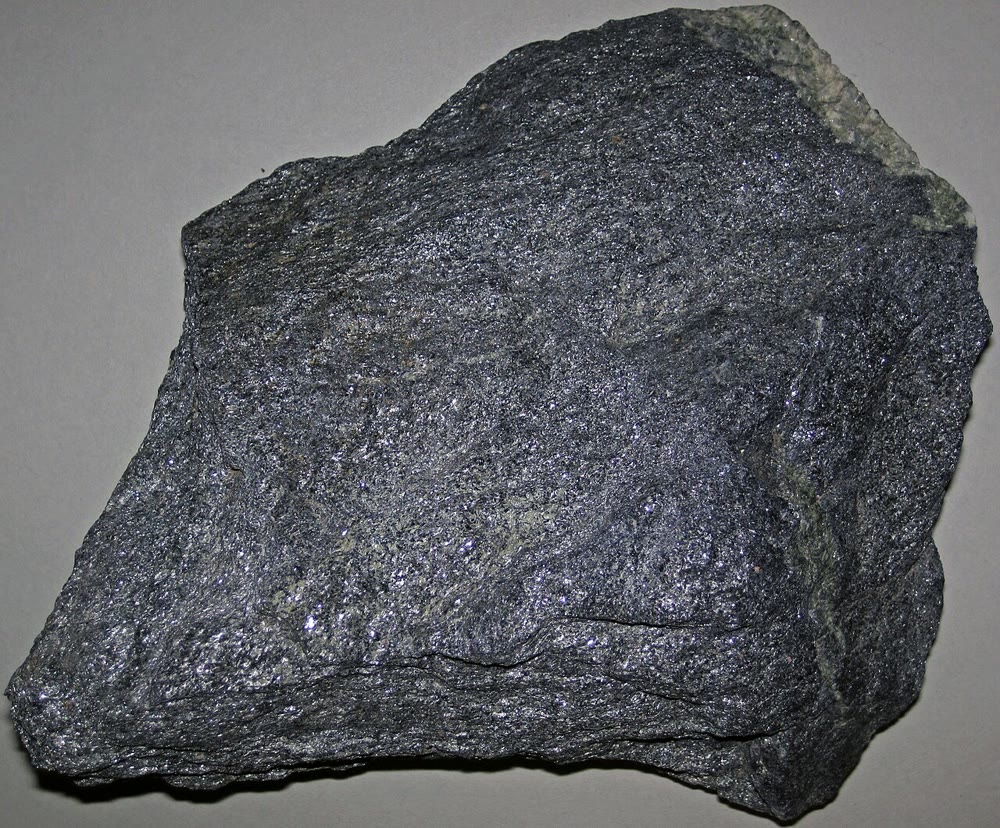
\includegraphics[width=0.27\linewidth]{images/book4/b2-10-blueschist.jpg}\hspace{0.02\linewidth}%
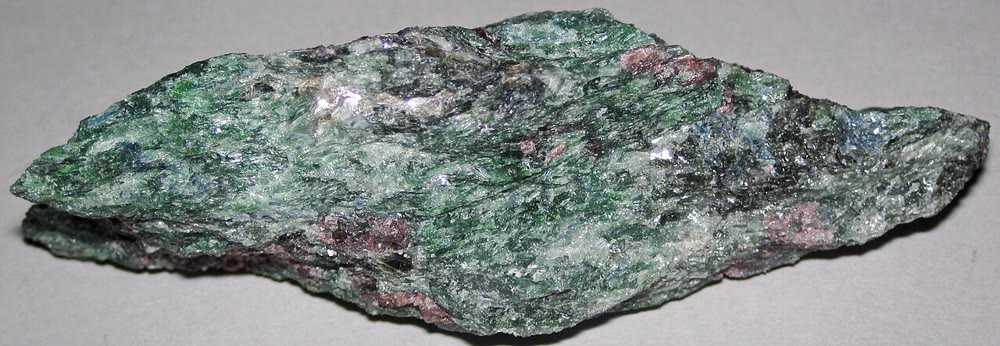
\includegraphics[width=0.69\linewidth]{images/book4/b2-10-eclogite.jpg}
\par\smallskip{\small 两块变质玄武岩。左：加利福尼亚弗朗西斯科杂岩中的硬柱石蓝片岩，
因含蓝闪石而呈蓝色。右：来自挪威西部的榴辉岩，
呈绿色的绿辉石和红色的石榴子石，并含少量石英、蓝晶石和金红石。
照片：James St.~John, CC BY 2.0。}
\end{omfigure}

一同埋藏并加热的岩石按规则的次序经过各\omterm{def:b2:metamorphic-facies:facies}{变质相}，这一次序
反映了其演化路径上压强与温度的比值：比值高时见于俯冲带，蓝片岩在此形成；
比值居中见于碰撞带；靠近侵入体时比值低。
\Cref{ch:b2:pt-paths}命名了这些系列，并从矿物中读出此类路径。
% ledger: scmr:facies

\section{原岩至关重要}\label{sec:b2:metamorphic-facies:protoliths}

\omterm{def:b2:metamorphic-facies:facies}{变质相}是在玄武岩上定义的，但每种\omterm{def:b2:metamorphic-facies:metamorphism}{原岩}
都在其自身矿物中记录了相同的条件。

\begin{definition}[变泥质岩；变基性岩]\label{def:b2:metamorphic-facies:protoliths}
称\emph{变泥质岩}\index{变泥质岩}为变质泥岩（泥质岩），富含
铝和钾，其\omterm{def:b2:metamorphic-facies:assemblage}{矿物组合}中含云母、绿泥石、石榴子石、十字石以及
铝硅酸盐矿物。\emph{变基性岩}\index{变基性岩}为变质玄武岩、
辉长岩或其他镁铁质岩石，富含钙、镁和铁，其\omterm{def:b2:metamorphic-facies:assemblage}{矿物组合}界定
\omterm{def:b2:metamorphic-facies:facies}{变质相}。
\end{definition}

在\omterm{def:b2:metamorphic-facies:protoliths}{变泥质岩}中，高中分册中的指示矿物随变质级升高依次出现
（绿泥石、黑云母、石榴子石、十字石、蓝晶石、夕线石），
本章中的白云母 + 石英反应在温度更高时生成夕线石和钾长石，
而存在的铝硅酸盐则指示岩石经过了三相点的哪一侧。
变质的石灰岩或白云岩变为大理岩，由方解石或
白云石组成；含硅质和黏土的不纯碳酸盐岩变为钙硅酸盐岩，其
脱碳反应释放二氧化碳；石英砂岩变为石英岩，
石英岩除粒度外几乎没有其他特征可显示。绿泥石带的一块\omterm{def:b2:metamorphic-facies:protoliths}{变泥质岩}及
其旁侧的一块变玄武岩，在相同压强和温度下，外观截然不同，后者
是由阳起石、绿泥石、绿帘石和钠长石组成的绿岩：一组条件，
两种\omterm{def:b2:metamorphic-facies:assemblage}{矿物组合}。
% ledger: iugs:barrow, day73:ms-qz, scmr:facies-assemblages

\section{练习}

\begin{exercise}[$\star$]\label{exo:b2:metamorphic-facies:1}
指出下列各情形属于何种\omterm{def:b2:metamorphic-facies:metamorphism}{变质作用}：(a) 石灰岩在
距花岗岩\qty{500}{m}范围内重结晶为大理岩；(b) 沿一条大型走滑
断层分布的细粒条带状岩石，其颗粒被压碎后又重结晶；(c) 洋壳中的玄武岩，其
玻璃质在洋脊附近已变为绿泥石和沸石，矿物仅部分被替代；(d) 火山砂岩位于
厚度为\qty{10}{km}的岩石堆底部，
重结晶但未形成片理。
\end{exercise}
% ledger: scmr:types

\begin{exercise}[$\star$]\label{exo:b2:metamorphic-facies:2}
由铝硅酸盐表，计算$\Delta_r S$、$\Delta_r V$以及蓝晶石$\to$夕线石的
\omterm{def:b2:metamorphic-facies:clapeyron}{克拉珀龙斜率}，分别以\unit{bar/K}和\unit{MPa/K}表示。
温度变化\qty{100}{\celsius}时，平衡压强改变多少？
\end{exercise}
% ledger: rh95:al2sio5

\begin{exercise}[$\star$]\label{exo:b2:metamorphic-facies:3}
下列各变玄武岩分别属于哪一\omterm{def:b2:metamorphic-facies:facies}{变质相}？(a) 阳起石、钠长石、绿泥石和绿帘石；
(b) 蓝闪石和硬柱石；(c) 角闪石和含\qty{30}{\percent}钙长石的斜长石；
(d) 绿辉石和石榴子石，不含斜长石。
\end{exercise}
% ledger: scmr:facies-assemblages

\begin{exercise}[$\star$]\label{exo:b2:metamorphic-facies:4}
(a) 由摩尔质量\qty{162.046}{g.mol^{-1}}以及摩尔体积44.15、51.52和
\qty{49.86}{cm^3.mol^{-1}}，计算蓝晶石、红柱石和夕线石的密度。
(b) 压强有利于哪一种多形体，为什么？(c) 矿物数据库给出的密度为3.61、3.15和
\qty{3.24}{g.cm^{-3}}：天然晶体为何可能与纯相不同？
\end{exercise}
% ledger: rh95:al2sio5, webmineral:polymorphs

\begin{exercise}[$\star\star$]\label{exo:b2:metamorphic-facies:5}
对于蓝晶石$\to$红柱石，$\Delta_r H = \qty{3.9}{kJ}$，$\Delta_r S =
\qty{8.59}{J.K^{-1}}$，$\Delta_r V = \qty{0.737}{J.bar^{-1}}$。(a) 在
\qty{25}{\celsius}、\qty{1}{bar}下哪一种多形体稳定？(b) 在\qty{1}{bar}下，两者于何温度
共存？(c) 计算\qty{400}{\celsius}时的平衡压强，
并与实验值\qty{2.54}{kbar}比较。(d) 为何红柱石
仍见于冷却至地表的岩石中？
\end{exercise}
% ledger: rh95:al2sio5, hm93:table11

\begin{exercise}[$\star\star$]\label{exo:b2:metamorphic-facies:6}
检验方法的第 (2) 步。在\qty{1000}{K}时，表中给出蓝晶石的$S_T$ = 285.02，
夕线石为296.44，以及$(H_T - H_{298})/T$ = 122.29和121.39
（\unit{J.mol^{-1}.K^{-1}}）。(a) 在\qty{1000}{K}、\qty{1}{bar}下计算该反应的
$\Delta_r H$、$\Delta_r S$和$\Delta_r G$（蓝晶石$\to$夕线石）；(b) 与表中
的常数值比较。(c) 此时哪一种多形体稳定，
简单方法的误差有多大？
\end{exercise}
% ledger: rh95:al2sio5-ht, rh95:al2sio5

\begin{exercise}[$\star\star$]\label{exo:b2:metamorphic-facies:7}
方解石与文石（\ce{CaCO3}）在\qty{298.15}{K}时，$\Delta_f G$ = $-1128.5$和
$-1127.4$ \unit{kJ.mol^{-1}}，$S$ = 91.7和88.0 \unit{J.mol^{-1}.K^{-1}}，$V$ = 36.93
和\qty{34.15}{cm^3.mol^{-1}}，且二者的生成焓相等。(a) 求
\qty{25}{\celsius}时的平衡压强。(b) 计算\omterm{def:b2:metamorphic-facies:clapeyron}{克拉珀龙斜率}。(c) 求
\qty{300}{\celsius}时的平衡压强。(d) 许多贝壳由文石构成，且生活在
\qty{1}{bar}下：这说明了什么？
\end{exercise}
% ledger: rh95:cc-ar

\begin{exercise}[$\star\star$]\label{exo:b2:metamorphic-facies:8}
对于钠长石$\to$硬玉+石英，表中给出$\Delta_r H = \qty{-5.0}{kJ}$，
$\Delta_r S = \qty{-32.4}{J.K^{-1}}$，$\Delta_r V = \qty{-1.698}{J.bar^{-1}}$。(a)
计算\omterm{def:b2:metamorphic-facies:clapeyron}{克拉珀龙斜率}。(b) 计算\qty{500}{\celsius}时的平衡压强。
(c) 钠长石、硬玉和石英的生成焓的不确定度分别为2.6、3.6
和\qty{1.0}{kJ.mol^{-1}}；若将其视为相互独立的误差进行合成，该压强的不确定度为多少？
(d) 为何榴辉岩相中缺少斜长石？
\end{exercise}
% ledger: rh95:ab-jd-qz, scmr:facies-assemblages

\begin{exercise}[$\star\star$]\label{exo:b2:metamorphic-facies:9}
白云母+石英在\qty{1}{kbar}、\qty{2}{kbar}和
\qty{3}{kbar}下分别于603、637和\qty{662}{\celsius}时分解。(a) 计算每两点之间连线的斜率。
(b) 若该范围内反应熵几乎不变，则从第一段到第二段，$\Delta_r V$
缩小了多少倍？(c) 哪一相是造成这一变化的原因？
\end{exercise}
% ledger: day73:ms-qz

\begin{exercise}[$\star\star\star$]\label{exo:b2:metamorphic-facies:10}
利用方法中的常数性质：(a) 计算三个反应在
\qty{600}{\celsius}时的压强；(b) 证明在\qty{600}{\celsius}、压强为
蓝晶石$=$红柱石时，夕线石是最稳定的多形体，
因此该点位于直线的亚稳态部分；(c) 在\qty{600}{\celsius}、
\qty{4}{kbar}以及\qty{600}{\celsius}、\qty{7}{kbar}下，各是哪一种多形体稳定？
\end{exercise}
% ledger: rh95:al2sio5

\begin{exercise}[$\star\star\star$]\label{exo:b2:metamorphic-facies:11}
一块片岩中蓝晶石、红柱石和夕线石共存，三者均
在平衡条件下生长。(a) 已知实验三相点为$504 \pm \qty{20}{\celsius}$和
$3.75 \pm \qty{0.25}{kbar}$，且地壳密度为\qty{2700}{kg.m^{-3}}（$g =
\qty{9.81}{m.s^{-2}}$），求其生长时的深度。(b) 取地表温度为\qty{10}{\celsius}，
由此推出平均地温梯度为多少？(c) 为何此类岩石十分罕见？
\end{exercise}
% ledger: hm93:triple

\begin{exercise}[$\star\star\star$]\label{exo:b2:metamorphic-facies:12}
两块岩石埋至深度$z$，地表温度为\qty{10}{\celsius}：岩石X沿
\qty{10}{\celsius.km^{-1}}升温至\qty{30}{km}深处，上覆岩石的平均密度为
\qty{3000}{kg.m^{-3}}；岩石Y沿\qty{30}{\celsius.km^{-1}}升温至\qty{20}{km}深处，
上覆岩石的平均密度为\qty{2800}{kg.m^{-3}}。(a) 计算每条路径末端的$T$和$P$。
(b) 利用常数性质的直线（方解石$=$文石：$P = 13.31\,T$ bar，其中$T$
以开尔文计；钠长石$=$硬玉+石英取自\cref{exo:b2:metamorphic-facies:8}；铝硅酸盐取自表中），
判断每块岩石含有的是文石还是方解石、硬玉+石英还是钠长石，以及
哪一种铝硅酸盐。(c) 哪条路径更冷、高压，两者分别终止于哪一\omterm{def:b2:metamorphic-facies:facies}{变质相}？
\end{exercise}
% ledger: rh95:cc-ar, rh95:ab-jd-qz, rh95:al2sio5

\section{问题：构造三相点}

\begin{problem}[{周末问题——由表格得到的铝硅酸盐图，以及该图
可信到何种程度}]
\label{pb:b2:metamorphic-facies:1}
利用铝硅酸盐表（\qty{298.15}{K}，\qty{1}{bar}）及
本章的方法，取 $\Delta_r H$、$\Delta_r S$ 和 $\Delta_r V$ 为常数；
$T$ 以开尔文计，$P$ 以 bar 计，并忽略 $P - 1$ 中的 1。

\noindent\textbf{第一部分——各反应。}
\begin{enumerate}
\item 计算 $\Delta_r H$、$\Delta_r S$ 和 $\Delta_r V$，反应为蓝晶石 $\to$ 红柱石。
\item 对蓝晶石 $\to$ 夕线石，做同样的计算。
\item 对红柱石 $\to$ 夕线石做同样的计算，并检验每个量都等于
前两个反应对应量之差。
\item 哪一种同质多象变体的熵最大，哪一种的体积最小？每种
同质多象变体将位于各条线的哪一侧？
\item 计算三条\omterm{def:b2:metamorphic-facies:clapeyron}{克拉珀龙斜率}。
\item 为什么红柱石 $\to$ 夕线石的斜率为负？
\end{enumerate}

\noindent\textbf{第二部分——各线的走向。}
\begin{enumerate}[resume]
\item 计算前两个反应在 \qty{298.15}{K} 时的 $\Delta_r G$。在地表
稳定的是哪一种同质多象变体？
\item 各反应在
\qty{1}{bar} 下达到平衡的温度（以 \unit{\celsius} 计）是多少？
\item 第~8~小题中的三个温度，哪些是稳定平衡，哪些
是亚稳态？（利用 \qty{1}{bar} 下三者的先后顺序。）
\item 计算蓝晶石 $=$ 红柱石在 \qty{400}{\celsius} 时的压强；
实验给出 \qty{2.54}{kbar}。
\item 计算蓝晶石 $=$ 夕线石在 \qty{700}{\celsius} 时的压强；
实验给出 \qty{7.86}{kbar}。
\item 画出 200 至 \qty{900}{\celsius} 之间三条线的示意图。
\end{enumerate}

\noindent\textbf{第三部分——三相点。}
\begin{enumerate}[resume]
\item 将前两条线写成 $P = a_i T - b_i$ 的形式，给出 $a_1$、$b_1$、$a_2$、$b_2$。
\item 求二者交点的温度。
\item 计算交点的压强。
\item 检验红柱石 $=$ 夕线石是否经过该点。
\item 与实验值 $504 \pm \qty{20}{\celsius}$ 及 $3.75 \pm
\qty{0.25}{kbar}$ 进行比较。
\item 若采用表中的温度依赖关系，三相点移至
\qty{536}{\celsius} 和 \qty{4.20}{kbar}。这一修正是否使结果更接近
实验？这说明误差的主要来源是什么？
\end{enumerate}

\noindent\textbf{第四部分——结果可信到何种程度。}
\begin{enumerate}[resume]
\item 将红柱石的生成焓提高 \qty{1}{kJ}，在温度不变时，
蓝晶石 $=$ 红柱石这条线的压强移动多少？
\item 三相点的温度移动多少？
\item 对夕线石的焓升高 \qty{1}{kJ} 的情形，做同样的计算。
\item 每个焓的不确定度均为 \qty{2.0}{kJ}。仅利用量热数据，
三相点温度的可能范围是多少？
\item 那么，热力学表格如何能将实验相图的再现误差控制在
\qty{30}{\celsius} 以内？
\item 给出第三部分中计算所得三相点的温度，四舍五入到
整数位，这是本题的关键数值。
\end{enumerate}
\end{problem}
% ledger: rh95:al2sio5, rh95:al2sio5-ht, hm93:triple, hm93:table11, hm93:adjusted
